\documentclass[conference]{IEEEtran}
%\IEEEoverridecommandlockouts
% The preceding line is only needed to identify funding in the first footnote. If that is unneeded, please comment it out.

\usepackage{cite}
\usepackage{amsmath,amssymb,amsfonts}
\usepackage{algorithmic}
\usepackage{graphicx}
\usepackage[hidelinks]{hyperref}
\usepackage{fontawesome}
\usepackage{textcomp}
\usepackage{xcolor}
\def\BibTeX{{\rm B\kern-.05em{\sc i\kern-.025em b}\kern-.08em
    T\kern-.1667em\lower.7ex\hbox{E}\kern-.125emX}}
\begin{document}

\title{Predicting Loan Defaulters\\
{\footnotesize Machine Learning Hackathon Report}
}

\graphicspath{{./images/}}

\author{\IEEEauthorblockN{Shobhit Behl}
\IEEEauthorblockA{\textit{IMT2016024}}
\and
\IEEEauthorblockN{Biswesh Mohapatra}
\IEEEauthorblockA{\textit{IMT2016050}}
\and
\IEEEauthorblockN{Aditya Hegde}
\IEEEauthorblockA{\textit{IMT2016054}}
}

\maketitle

\begin{abstract}
The aim of the project is to successfully predict whether a loan would
default. We used the dataset provided by Lending Club which is a
peer-to-peer lending company. The dataset is available in Kaggle at
\href{https://www.kaggle.com/wendykan/lending-club-loan-data}{lending-club-loan-data\hspace{0.5em}\faExternalLink}
\end{abstract}

\section{Introduction}
In this project we try to analyze the dataset provided by LendingClub to try
and build a model for predicting which loans would default. The dataset was
extremely rich, consisting of a lot of attributes and a significant amount of
our time involved their analysis. We ended up doing reasonably well with respect
to our performance metric considering the constraints.

\section{Data}
To label the dataset we derived a new attribute called ‘defaulter’ from the
existing ‘loan\_status’ attribute. This step was necessary since the
‘loan\_status’ attribute contained multiple categories but our model needed to
only predict if a loan would result in a default or not. Hence we combined
negative attributes of ‘loan\_status’ like `charged off', `late' and `default'
under a ‘defaulter’ label of -1 and some positive ones like `current' and
`fully paid' under a `defaulter’ label of 1. We dropped rows (\textasciitilde 14000 of out
of 8 lakhs) having a `loan\_status' of `issued' or `in grace period' since
these labels weren't associated with a positive or negative aspect.

\subsection{Feature Extraction}
As this is a general purpose dataset, there were many features which were not
required for our model. We initially went through the data dictionary provided
with the dataset and removed 18 attributes which we felt weren't related to the
label prediction. This also included attributes like `late\_fee' and
`recovery\_fee' that are not available when a loan is first offered but have
strong correlation with the label. Such attributes might lead to good results
but the model wouldn't be useful since it wouldn't actually be predicting the
labels.

We also decided to remove attributes that had at least 10\% null values
(\textasciitilde 90,000 rows). This left us with around 35 columns which we felt
might contribute to the model.

\subsection{Feature Analysis}
Some attributes like `loan\_amount', `annual\_income' etc.\ were obviously
important for predicting the label. Thus, our analysis was focussed around those
attributes we weren't sure about.

Analysis of the label showed that the dataset was extremely skewed. The number
of defaulters were only 61,000 compared to 8,11,000 non-defaulters. This led to
a huge increase in the complexity of the problem.

\begin{figure}[ht]
    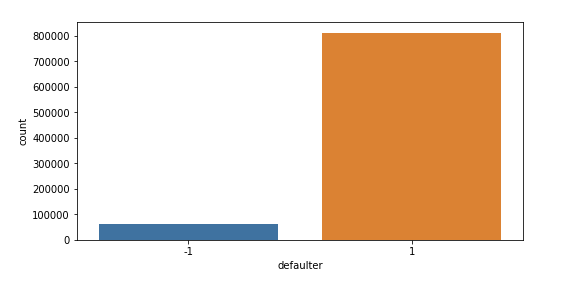
\includegraphics[width=\columnwidth]{defaulter_skew}
    \caption{Skew in label}
\end{figure}

Analysis of the columns mainly revolved around getting its relationship with
`defaulter'.
\begin{itemize}
    \item {\bf collections\_12\_mths\_ex\_med}: The column conveyed the number
        of collections in 12 months excluding medical collections. It turned
        out to be highly skewed as the majority of the values were 0 and the
        remaining values resulted in only 604 defaulters. Hence we decided
        to drop the attribute.

    \item {\bf dti}: Although the column contains `debt-to-income-ratio' of
        the borrower, a basic analysis didn't seem to show any direct relation.
        We decided to further analyze the feature when building the model.

    \item {\bf funded\_amnt}: Again, the values of the attribute when seen
        after grouping by the ‘Defaulter’ attribute, were distributed similarly.
        Hence the feature didn’t contribute much to the final prediction.

    \item {\bf initial\_list\_status}: The column contained information about
        whether the loan was given as a fraction(f) or as a whole(w). We
        noticed that the probability of being a defaulter is slightly more in
        the case of fractional loans ('f') than whole loans ('w'). This feature
        seemed to be useful considering our skewed dataset.

        \begin{figure}[ht]
        \center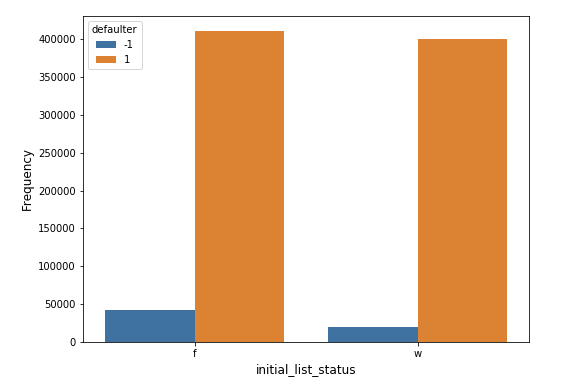
\includegraphics[scale=0.3]{initial_list_status}
            \caption{The number of defaulters is significantly more in fraction type loans}
        \end{figure}

    \item {\bf int\_rate}: This feature seemed to be important since a higher
        interest rate corresponded to a higher frequency of defaulters as
        shown by the data.

        \begin{figure}[ht]
        \center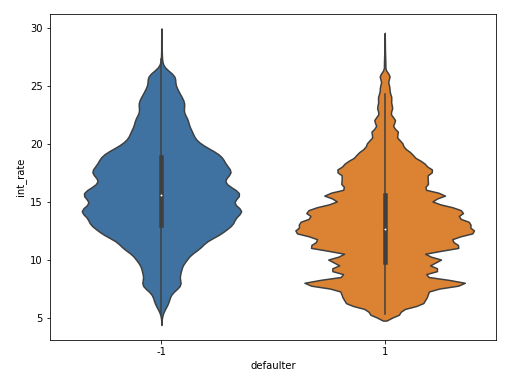
\includegraphics[scale=0.3]{int_rate}
            \caption{Higher interest rates correspond to more defaulters}
        \end{figure}

    \item {\bf policy\_code}: The attribute gave information about the loan
        policy and seemed to be very important. But we realised that the entire
        dataset contained only 1 type of policy code and hence decided to drop
        it.

    \item {\bf pub\_rec}: The feature conveyed the previous public offence
        record of the borrower. The probability of a defaulter given the
        pub\_rec value didn't seem to be much different than just the
        probability of the class. Hence we decided to drop the column.

    \item {\bf pymnt\_plan}: The feature conveyed if the borrower had submitted
        any plans of repayment of the loan. Although the feature seemed
        important since a plan would translate to greater confidence in the
        borrower. Unfortunately, the data was highly skewed and we had only
        10 people who had submitted a plan. Hence we had to remove this
        feature as well.

    \item {\bf sub\_grade}: The attribute told us about the grade associated
        with the loan. Our analysis showed that the ratio of defaulters increases
        significantly with decrease in grade making the column extremely important
        for building the model.

        \begin{figure}[ht]
        \center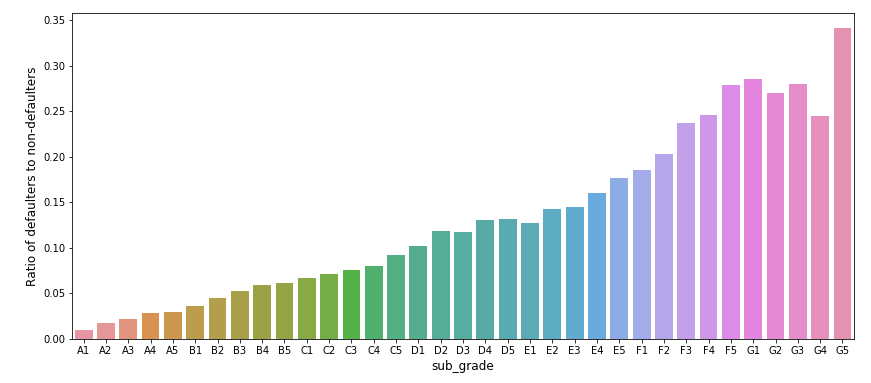
\includegraphics[scale=0.3]{sub_grade}
            \caption{Direct relation between sub\_grade and defaulters}
        \end{figure}

    \item {\bf application\_type}: The column value denoted whether
        the loan was taken jointly or by an individual. Unfortunately,
        the dataset had only 400 joint loans. Hence the attribute was highly
        skewed an could not be used.

    \item {\bf delinq\_2yrs}: The column values were the number of 30+ days past-due
        incidences of delinquency in the borrower's credit file for the past 2
        years. The probability of a default loan conditioned on delinq\_2yrs
        was almost the same as just the probability of a defaulter, suggesting
        that the information gain was negligible. Hence we decided to drop the
        column.

    \item {\bf purpose}: The feature showed the motive behind the loan. The
        probability of defaulters conditioned on purpose was quite high which
        indicated that this was an important column.

        \begin{figure}[ht]
        \center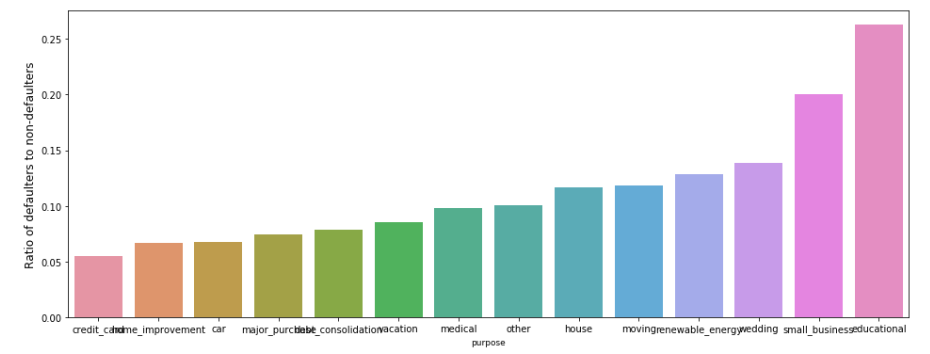
\includegraphics[scale=0.3]{purpose}
            \caption{Relation between purpose and defaulters}
        \end{figure}
\end{itemize}

Our exploratory data analysis notebook consists of analysis of more features.
We also used metrics like feature importance provided by Random Forest and
lightgbm to further improve the feature set.

\section{Evaluation Metrics}
From an application perspective, it's costlier to incorrectly classify a loan
that will default. It would be preferable if our model was able to identify all
defaulters with good accuracy. Moreover, accuracy is not a good measure for
skewed datasets since the model just doesn't have enough information to predict
classes accurately. Keeping this in mind, we felt that Sensitivity
would be a good measure

\begin{equation*}
    \text{sensitivity} = \frac{TP}{(TP + FN)}
\end{equation*}

Henceforth defaulters will be considered as `positives' while non-defaulters
will be considered as `negatives'. This is just an arbitrary labelling to make
the analysis easier.

Sensitivity is the ratio of correctly predicted defaulters to the actual
defaulters. Having sensitivity as the only measure is not enough since we
aren't capturing the number of incorrectly classified defaulters. Precision is
a good measure to capture this

\begin{equation*}
    \text{precision} = \frac{TP}{(TP + FP)}
\end{equation*}

Precision is essentially the ratio of correctly predicted defaulters to the
total number of predicted defaulters. Clearly, there's a trade-off between
precision and recall and ideally we would like to maximize both. However,
this turns into a harder problem in case of a skewed dataset like the Lending Club
data.

\section{Models}
Due to the large number of important categorical columns, we tried to select a
good feature set by observing the metrics output by estimators e.g.\
feature\_importance by Random Forest.

We had divided the dataset into training and test sets in a 70-30 ratio before
building any of the models. Every model was initially built using a part of
the training data and the other part was used for validation. The model that
gave the best validation score was run against the test set.

\subsection{Ensemble Models}
Since Random Forests are known to give good accuracy when trained on correlated
attributes (compared to other models) we started off with it. But the time taken
to train each Random Forest made us turn towards LightGBM\@. We found that LightGBM
gave similar accuracy as Random Forest and XGBoost but was an order efficient
with respect to time.

Our earliest approaches involved using basic numerical features for building the
model. Unfortunately, it gave a sensitivity of 0.5 and precision of 0.03. Using
other features didn't lead to significant improvement.

We realized that the scores were low due to the skew. We tried to balance the
training data by having almost same number of defaulters and non-defaulters.
This led to considerable improvement of sensitivity to 0.75 and precision to
0.18.

We now had a hyper-parameter i.e.\ the ratio of defaulters to non-defaulters in
training data. A bit of exploration and testing suggested that having equal
distribution of defaulters led to a good balance between sensitivity and
precision.

Our next approach involved training on different subsets of features that we
had analyzed during EDA. We observed that certain columns like `state\_address'
and `emp\_title' didn't improve the score. Also, features like `dti' that we
were doubtful about gave a good boost to the score.

Multiple iterations of the above approach finally led us to a sensitivity of
0.843 and a precision of 0.214 during validation.

\subsection{Naive Bayes}
Since generative models tend to perform better on small data sets we thought
training a Naive Bayes model on an equally distributed training set would give
good validation score. The model gave a sensitivity of 0.76824 but the precision
was 0.118.

\subsection{Logistic Regression}
Logistic regression gave a sensitivity of 0.62 and a precision of 0.28 on the
validation set. Since, we required the sensitivity to be significantly higher
than 0.5 we felt that the ensemble models performed better.

\section{Conclusion}
We finally chose the LightGBM model which had given a sensitivity of 0.843 and
a precision of 0.214 during validation as the final model. Upon predicting
against the test set, we got the following results

\smallskip
\begin{center}
\begin{tabular}{ |l|r| }
 \hline
 Sensitivity & 0.8633 \\
 Precision & 0.2212 \\
 Specificity & 0.769 \\
 Accuracy & 0.776 \\
 \hline
\end{tabular}
\end{center}

Thus the test score was quite close to the validation score. We thus have a
reasonable and consistent model.
\end{document}
